\section{Succinct Solver}
The succinct solver is a blackbox approach to solve the exact same problems as we have solved with our own implementation. The succinct solver uses Alternation-Free Least Fixed Point Logic (ALFP) to describe the problem and how it should be solved. ALFP is described as follows:

Values:
$v ::= c | x | f(v_1,...,v_k)$

Preconditions:
$pre ::= R(v_1,...v_k) | \neg R(v_1,...,v_k)
      |  v_1 = v_2 | v1 \not= v_2
      |  pre_1 \wedge pre_2 | pre_1 \vee pre_2
      |  \forall x : pre | \exists x : pre$

Clauses:
$cl ::= R(v_1,...,v_k) | true | cl_1 \wedge cl_2
     |  pre \Rightarrow cl | \forall x : cl$

For our test of the succinct solver, we are only going to use RDA for comparison. Additional analysis could be formed using the above clauses if time had permitted it.

\subsection{Succinct solver correctness}
To see the actual clauses in action, the following example can be used. But before the walkthrough of an example, there is a small disclaimer. The clauses generated may not be perfect (as in, formed such that it would help the succinct solver), but immitates the internal representation of everything. This means that temporary variables might occure in the resulting set og clauses which they are not visible in the code from which it is generated from. Also, the labeling does not start from 1 and counts up, but uses the hashcodes of statements that is also used internally.

This is a simple program:
\begin{lstlisting}
module example:
read x;[4d47c5fc]
read y;[4e3eca90]
x := 1;[19c1ea29]
y := (x+2);[4413ee]
write (y);[3597a37c]
\end{lstlisting}
The generated set of clauses will then be:

var(x) \& var(y) \&\newline
label(0) \& label(19c1ea29) \& label(3597a37c) \& label(4413ee) \& label(4d47c5fc) \& label(4e3eca90) \&\newline
flow(4e3eca90,19c1ea29) \& flow(4d47c5fc,4e3eca90) \& flow(4413ee,3597a37c) \& flow(19c1ea29,4413ee) \& flow(0,4d47c5fc) \&\newline
(A lab. label(lab) $\Rightarrow$ kill(4e3eca90,y,lab)) \& (A lab. label(lab) $\Rightarrow$ kill(4413ee,y,lab)) \& (A lab. label(lab) $\Rightarrow$ kill(4d47c5fc,x,lab)) \& (A lab. label(lab) $\Rightarrow$ kill(19c1ea29,x,lab)) \&\newline
gen(4e3eca90,y,4e3eca90) \& gen(4413ee,y,4413ee) \& gen(4d47c5fc,x,4d47c5fc) \& gen(19c1ea29,x,19c1ea29) \&\newline
(A lab. A x. A d. var(x) \& label(d) \& (RDentry(lab,x,d) \& ! kill(lab,x,d)) $|$ gen(lab,x,d) $\Rightarrow$ RDexit(lab,x,d)) \&\newline
(A lab1. A lab2. A x. A d. flow(lab1,lab2) \& RDexit(lab1,x,d) $\Rightarrow$ RDentry(lab2,x,d)) \&\newline
(A x. var(x) $\Rightarrow$ RDentry(4d47c5fc,x,0))

var(x) and var(y) tells the solver, that there exists a variable named x, and a variable named y. Label() tells the solver that this label exists in the program. flow() tells the solver how to move through the program, the first value listed inside flow() is where to move from, and the last value is where to move to. For the clauses for kill(), it requires a bit more concentration. For all lab in label(lab) (all labels which have been defined by label(x)), kill the variable y that have been defined at lab, on label z. The first value of kill() is where the kill is taken place, the second value is the variable, and the third value is where the variable were assigned (and where it was generated). For gen(), the first value tells where the generation takes place, the second is the variable generated, and the last value is where the variable is generated (so the first and the last value will be the same). The next two lines is what actually makes this a RDA. It tells the solver how to handle all these clauses above, how it should move through the flow of labels, and how gen and kill should be interpreted. The last line sets the entry value for the first statement in the code, setting all variables as coming from statement 0 (unknown).

Supplying that to the succinct solver will result with the following (we are only interested in RDentry and RDexit, not all the other values it outputs):

\begin{center}
	\begin{tabular}{ | c | c | }
		\hline
		RDentry & RDexit \\
		\hline
		\hline
		(4d47c5fc,x,0),(4d47c5fc,y,0) & (4d47c5fc,x,4d47c5fc),(4d47c5fc,y,0) \\
		(4e3eca90,x,4d47c5fc),(4e3eca90,y,0) & (4e3eca90,x,4d47c5fc),(4e3eca90,y,4e3eca90) \\
		(19c1ea29,x,4d47c5fc),(19c1ea29,y,4e3eca90) & (19c1ea29,x,19c1ea29),(19c1ea29,y,4e3eca90) \\
		(4413ee,x,19c1ea29),(4413ee,y,4e3eca90) & (4413ee,x,19c1ea29),(4413ee,y,4413ee) \\
		(3597a37c,x,19c1ea29),(3597a37c,y,4413ee) & (3597a37c,x,19c1ea29),(3597a37c,y,4413ee) \\
		\hline
	\end{tabular}
\end{center}

So the analysis concludes, that the value of x after the last statement comes from an assignment at label 19c1ea29, while the value of y comes from label 4413ee. Checking this with the program confirms the conclusion.

Next is for our analysis. This is the output of the analysis:

\begin{lstlisting}
module example:
read x;		//ID: 4d47c5fc, Analysis: [x = 4d47c5fc; y = 0]
read y;		//ID: 4e3eca90, Analysis: [x = 4d47c5fc; y = 4e3eca90]
x := 1;		//ID: 19c1ea29, Analysis: [x = 19c1ea29; y = 4e3eca90]
y := (x+2);		//ID: 4413ee, Analysis: [x = 19c1ea29; y = 4413ee]
write (y)		//ID: 3597a37c, Analysis: [x = 19c1ea29; y = 4413ee]
end
\end{lstlisting}

The ID is the label for that statement. Analysis is whatever is the exit value of the evaluation. At the last statement, it concludes that x comes from label 19c1ea29 and y comes from label 4413ee, which is exactly the same the analysis using the succinct solver. So for simple statements, the conclusion is the same.

For more advanced statements, both the flow and the results of RDentry and RDexit gets a lot more hairy to check. There are several other tests in appendix 7.1 to 7.5.

\subsection{Succinct solver speed}
Solving RDA, or any other analysis for that matter, requires a balance between the time it can take, and the precision of the calculations. Getting a very precise result will take extra time to complete. Shifting for a more unprecise solution will reduce the time, but how close can the calculations be moved towards being unprecise, and still get the correct result? That can be an entire study for itself, and is not going to be explored here. This section is for exploring the speed of the given succinct solver, and compare it with our solution.

The approach is as follows: a base program is going to be used, and then for each test, a new section is added. The new section does not necessarily have to be complicated, it can be as simple as a couple of assign statements. The base program will be this:
\begin{lstlisting}
module speed_test:
read x;
read y;
y := y + x;
x := x + y;
do x < y -> x := x + 1
[] y < x -> y := y + 1
od;
write y;
write x
end
\end{lstlisting}
The section added will be the same as the assign statements after the two read:
\begin{lstlisting}
y := y + x;
x := x + y;
\end{lstlisting}
And it will be added right after the do-statement.

The succinct solver have two different algorithms for solving the clauses implemented. A differential algorithm, and a BDD based algorithm. This test will use both of them, and to help them as much as possible, each execution will be done a couple of times to get the time when the kernel have the clauses cached.

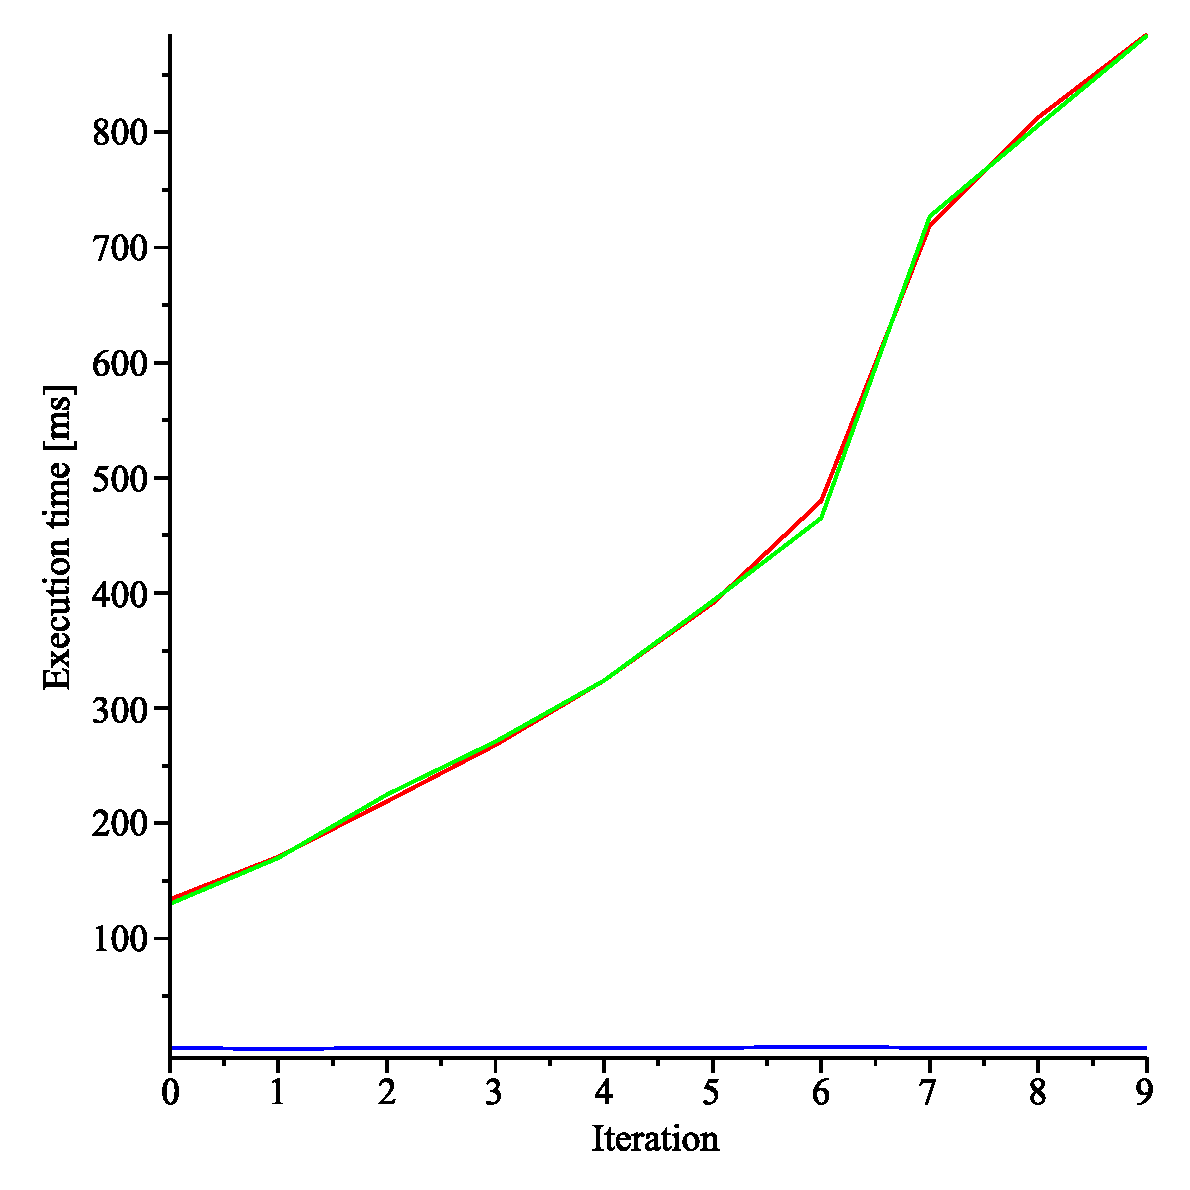
\includegraphics[width=1\textwidth]{alfp_graph.eps}

The red line executions times for the differential algorithm, the blue line is our implementation, and the green line is the BDD based algorithm. The values can be seen in appendix 7.6.

As the graph shows, the time for our implementation is very close to constant in this test, while the time for both algorithms rises. Something strange happens between execution 7 and 8, as the time jumps with just over 200 ms. It was also about that point where it took up to 10 executions before the time were as low as those in the graph. Instead, the execution time would be somewhere from 1000 ms to 4000 ms, and usually about 1400 ms. Perhaps the size of storing the calculations which needed to be done on the clauses, became higher than what the kernel wanted to cache, and therefore it had to load in the rest of the calculations before it could continue. Perhaps it had to rehash everything because the number of clauses where higher than there were space for. No matter what the reason is, the use of the succinct solver is still the slowest solution to use.

